\section{Condizioni di applicabilità}
\label{sec:chapter_lrl_cond_app}

Il lightweight render loop permette di diminuire drasticamente le operazioni effettuate dal ciclo di render quando viene calcolata una scena in cui sono presenti un elevato numero di luci e superfici riflettenti/rifrangenti. 
L’utilizzo delle informazioni di luci ed ombre precalcolate e salvate su lightmap e l’utilizzo delle env-map di riflessione e rifrazione è però possibile solo su scene statiche e immutabili nel tempo.
Modificare una scena dopo che sono state applicate delle lightmap e delle env-map porterebbe ad un risultato fisicamente impossibile da osservare nella vita reale. 
È preferibile infatti evitare di modificare la posizione di oggetti che proiettano ombra su una scena in cui il bake è già stato effettuato in quanto l’ombra non si sposterebbe dinamicamente insieme all’oggetto. Essa piuttosto rimarrebbe fissa nella vecchia posizione. 
Inoltre l’oggetto spostato non proietterebbe nessuna ombra nella nuova posizione, rendendo di fatto la scena renderizzata non realistica. 
\\
\begin{figure}[htb]
 \centering
 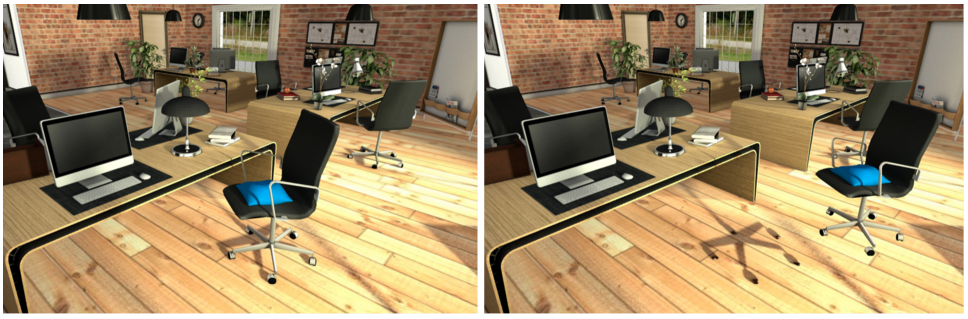
\includegraphics[width=1\linewidth]{images/chapter_lrl/lrl_appl1.png}\hfill
 \caption[Applicabilità, ombre statiche]{In foto è mostrato l'effetto del processamento offline delle informazioni luminose. L' ombra sul pavimento rimane statica anche dopo lo spostamento dell'oggetto che l'aveva proiettata.}
 \label{fig:lrl_appl1}
\end{figure}
Questo inconveniente viene ottenuto perchè le informazioni di luci ed ombre sono salvate all’interno delle lightmapped texture, ed all’interno del ciclo di render non viene effettuato alcun calcolo dinamico delle luci  (perchè le luci sono totalmente assenti nella scena).
Stesso discorso per le env-map, modificare la scena dopo che le env-map sono state calcolate renderebbe irrealistici gli effetti di riflessione e rifrazione. Questo perchè le superfici continuerebbero a riflettere o rifrangere  il vecchio ambiente che risulterebbe diverso da quello modificato.
\\
\begin{figure}[htb]
 \centering
 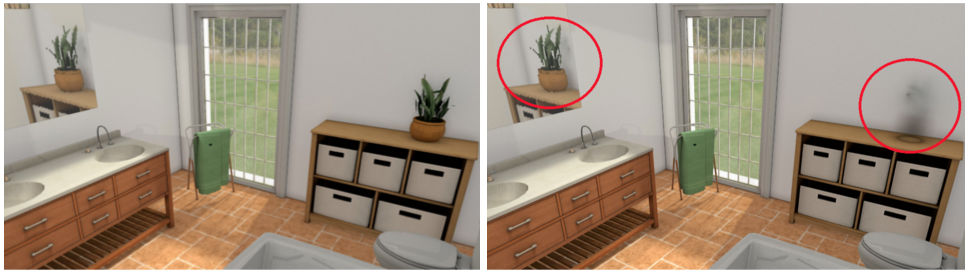
\includegraphics[width=1\linewidth]{images/chapter_lrl/lrl_appl2.png}\hfill
 \caption[Applicabilità, riflesso con env map]{Uno specchio ottenuto tramite una env map riflettente. Il riflesso risulta però immutibile nonostante lo spostamento degli oggetti.}
 \label{fig:lrl_appl2}
\end{figure}
Proprio per questi motivi è possibile ottenere scene fotorealistiche e scalabili solamente se esse, una volta create, non vengono modificate nel tempo.
\\
Questo di fatto non rappresenta una limitazione per il presente lavoro di tesi in quanto l’applicazione creata è rivolta principalmente ad architetti per la creazione di appartamenti fotorealistici.
\\
Gli appartamenti infatti una volta progettati ed arredati risultano completamente statici nel tempo in quanto in essi sono totalmente assenti animazioni, come lo spostamento di un oggetto.
\\
Quindi per l’architetto è sufficiente creare l’appartamento, scegliere da dove provengono le luci, inserire gli effetti di riflessione/rifrazione ed avviare il processo di bake.
Siccome questi effetti così come le luci influenzano l’intero appartamento, esattamente come nel mondo reale, è necessario che la scena creata sia completamente computata durante il processo di bake. 
\\
Se ad esempio venisse processato un bake diverso per ogni singola stanza, il risultato ottenuto non risulterebbe completamente corretto in quanto luci ed ombre posso conivolgere insieme più stanze e gli effetti di riflessione/rifrazione in una stanza possono dipendere da altre stanze.
\\
\begin{figure}[htb]
 \centering
 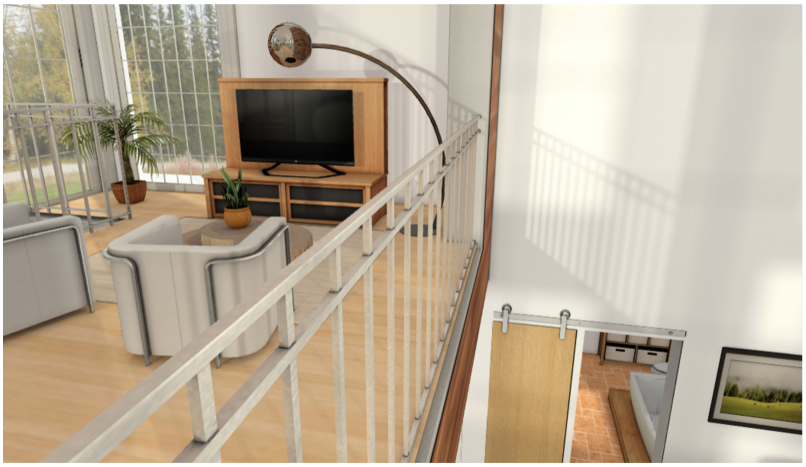
\includegraphics[width=1\linewidth]{images/chapter_lrl/lrl_appl3.png}\hfill
 \caption[Applicabilità, scene autocontenute]{Effetti di luce fotorealistici ottenuti tramite un unico bake dell'intera scena.}
 \label{fig:lrl_appl3}
\end{figure}
Questo ragionamento può essere applicabile solo su porzioni di scena autocontenute, come ad esempio una stanza chiusa di un appartamento, in cui è impossibile che luci, ombre ed effetti di riflessione/rifrazione possano influenzare altre stanze.
Nulla vieta comunque l’applicazione totale o parziale di questa tecnica su scene dinamiche, in cui il beneficio ottenuto dal miglioramento delle prestazioni è talmente elevato da giustificare  risultati non completamente realistici. 